\documentclass[openany,12pt]{book}

\usepackage{minted}
\usepackage{generalsnips}
\usepackage{programmingsnips}
\usepackage[left=1cm,right=1cm,top=1cm,bottom=1.5cm]{geometry}
\usepackage{pdfpages}
% \usepackage[spanish]{babel}
\usepackage{amsmath}
\usepackage{amsthm}
\usepackage[utf8]{inputenc}
\usepackage{titlesec}
\usepackage{lmodern}
\usepackage{xpatch}
\usepackage{fancyhdr}
\usepackage{fancyvrb}
\usepackage{tikz}
\usepackage{hyperref}
\usepackage{enumitem}
\usepackage{supertabular}
\usepackage{spverbatim}
\usepackage{fvextra}
\usepackage{listings}

\title{Complete Python Boot camp — Go from zero to hero in Python 3 }
\date{2020 May 18} % , 11:16AM
\author{David Corzo}
\darktheme
\pagestyle{plain}
\newcommand{\code}{./Code}

\begin{document}
\maketitle
\tableofcontents
%%%%%%%%%%%%%%%%%%%%%%%%%%%%%%%%%%%%%%%%%%%%%%%%%%%%%%%%%%%%%%%%%%%%%%%%%%%%%%%%%%%%%%%%%%%%%%%%%%%%%%%%%%%%%%%%%%%%%%%%%%%%%%%%%%%%%%%%%%%%%%
\chapter{Python Object and Data Structure Basics}
\section{What beginners don't know}
\begin{itemize}
    \item Command line basics: 
        \begin{itemize}
            \item Windows, macOS, Linux 
        \end{itemize}
    
    \item Installing python and making it a path environment variable. 
    \item Difference between distributions.
    \item How to google search for answering one's own questions. 
    \item How to run python code. 
    \item Difference between an IDE and python. 
    \item What is syntax highlighting. 
    \item Variables and their purpose. 
\end{itemize}


%----------------------------------------------------------------------------------------

\section{Basic data types}
\begin{center}
    \begin{tabular}{ |l|l| }
        \hline
            Name & Type  \\
        \hline
            Integers & int \\ 
        \hline
            Floating point & float \\ 
        \hline
            Strings & str \\ 
        \hline
            Lists & list \\ 
        \hline
            Dictionaries & dict \\ 
        \hline
            Tuples & tup \\ 
        \hline
            Sets & set \\ 
        \hline
            Booleans & bool \\ 
        \hline
    \end{tabular}
\end{center}


%----------------------------------------------------------------------------------------
\section{Numbers}
\begin{center}
    \begin{tabular}{ |p{5cm}|p{5cm}|p{5cm}| }
        \hline\\[0.25cm]
            Modulo & 20 \% 2 & $\displaystyle 20\times\pmod{2}$  \\[0.45cm]
            \hline
            Powers & 2 ** 2  & $\displaystyle 2^2$  \\[0.45cm]
            \hline
            Floor & 10 // 3  & $\displaystyle \floor{\frac{10}{3} } $  \\[0.45cm]
            \hline
            Grouping & (10 + 3) / 3 & $\displaystyle \frac{10+3}{3} $ \\[0.45cm] 
        \hline
    \end{tabular}
\end{center}

%----------------------------------------------------------------------------------------
\section{Variable names}
Rules: 
\begin{itemize}
    \item No spaces 
    \item Can't use these: \mintinline{python}{;"',<>\()!@#$%^&*~-+|}
    \item Don't use keywords. 
\end{itemize}
\subsection{Dynamic typing}
\begin{itemize}
    \item Python is a dynamically typed language.
    \item This means you can reassign variables to different data types. 
    \item This makes Python very flexible in assigning data types, this is different to other languages that are ``Statically-Typed''.
\end{itemize}
\begin{center}
    \begin{tabular}{ |p{8.5cm}|p{8.5cm}| }
        \hline
            Pros & Cons \\
        \hline
            \begin{itemize}
                \item Easy to work with
                \item Faster development process 
            \end{itemize}
            & 
            \begin{itemize}
                \item May result in bugs for unexpected data types.
                \item You need to be aware of \verb|type()| function to check this. 
            \end{itemize}
            \\ 
        \hline
    \end{tabular}
\end{center}



%----------------------------------------------------------------------------------------
\section{Strings}
\begin{itemize}
    \item In Python ' and " are the same in strings. 
    \item String indexing: used to extract a single character in a string. a[index] 
    \item String slicing: grabs an interval of indexes. a[start:stop:step]
        \begin{itemize}
            \item start: numerical index for the slice start. 
            \item stop index you will go up to but not include. 
            \item step: the size of the jump you take. 
        \end{itemize}
    
    \item Special characters: \verb|\n, \t, \d|
    \item the lenght function: len(a) -$>$ how many elements are in the string. 
\end{itemize}
\subsection{Normal and reverse indexes}
\begin{center}
    \begin{tabular}{ |l|l|l|l|l|l|l|l|l|l|l|l|l| }
        \hline
            H & E & L & L & O &   & W & O & R & L & D & ! \\
            \hline
            0 & 1 & 2 & 3 & 4 & 5 & 6 & 7 & 8 & 9 & 10 & 11 \\ 
            \hline
            0 & -11 & -10 & -9 & -8 & -7 & -6 & -5 & -4 & -3 & -2 & -1 \\ 
        \hline
    \end{tabular}
\end{center}
\subsection{Examples}
\begin{minted}[autogobble]{python}
    # STRING INDEXES AND REVERSE INDEXES
    a = "123456"
    a[1:2] 
    # output: "2" -> Index 1 up to but not including 2
    a[1:3]  
    # output: "23" -> Index 1 up to but not including 3
    a[:3]   
    # output: "123" -> Index 0 (default) up to but not including 3
    a[::]   
    # output: "123456" -> Normal string 
\end{minted}


%----------------------------------------------------------------------------------------
\section{String properties}
\begin{itemize}
    \item Strings are inmutable: 
        \begin{minted}[autogobble]{python}
            name = "david"
            name[0] = "b" 
            # OUTPUT: 
            # Traceback (most recent call last):
            #   File "<stdin>" line 1, in <module>
            # TypeError: 'str' object does not support item assignment
        \end{minted}

        
    
    \item You can concactenate using the + and * signs
        \begin{minted}[autogobble]{python}
            2 + 3 
            # output: 5
            "2" + "3" 
            # output: "23"
            "h" * 10 
            # output: "hhhhhhhhhh" 
        \end{minted}
    
    \item Methods: 
        \begin{itemize}
            \item .upper()
            \item .lower()
            \item .replace()
            \item .split()
        \end{itemize}
\end{itemize}


%----------------------------------------------------------------------------------------
\section{Print formating with strings}
\begin{itemize}
    \item .format() for string interpolation:
        \begin{minted}[autogobble]{python}
            print("this is a string {}".format("inserted"))
            # output: This is a string inserted

            print("The {} {} {}".format("fox","brown","quick"))
            # output:  The fox brown quick 

            print("The {2} {1} {0}".format("fox","brown","quick"))
            # output: The quick brown fox

            print("The {a} {b} {c}".format(a="fox",b="brown",c="quick"))
            # output: The quick brown fox

            result = 100/777
            print(result) 
            # output: 0.1287001287001287
            # Float formatting formula "{value:width.precision f}"
            print("The result was {r:1.3f}".format(r=result))
            # output: The result was 0.129 
        \end{minted}

    \item f-strings for string interpolation: 
        \begin{minted}[autogobble]{python}
            # F-STRING FORMATING
            var = "World"
            print(f"Hello {var}")
            # output: Hello World
        \end{minted}
\end{itemize}

%----------------------------------------------------------------------------------------
\section{Lists}
\begin{itemize}
    \item They suport indexing and slicing.
        \begin{minted}[autogobble]{python}
            my_list = [1,2,3] 
            my_list[1:]
            # output: [2,3]
            another_list = [4,5]
            my_list + another_list 
            # output: [1,2,3,4,5]
        \end{minted}
        
    \item You can also concactenate lists together. 
    \item Lists are mutable. 
\end{itemize}
\subsection{Methods}
\begin{itemize}
    \item .append(\placeholder{something}) -$>$ Appends to the list. 
    \item .sort() -$>$ sorts the iterable alphabetically or numericaly, this is a void, it doen't return anything, don't assign it to anything because it returns None.
        \begin{minted}[autogobble]{python}
            new_list = ['a','e','x','b','c']
            new_list.sort()
            new_list
            # output: ['a','b','c','e','x']
        \end{minted}
        
    \item .pop() $\rightarrow$  eliminates last element and prints it.
        \begin{minted}[autogobble]{python}
            my_list.pop(0) 
            # output: pops element 0.
        \end{minted}
        
    \item .reverse() $\rightarrow$ returns the reverse of the list. 
\end{itemize}

%----------------------------------------------------------------------------------------
\section{Dictionaries}
\begin{itemize}
    \item Doesn't need indexes. Just keys and values. 
    \item Dictionaries are unordered and can't be sorted.
    \item Methods:
        \begin{minted}[autogobble]{python}
            d = {"key1":1,"key2":2}
        \end{minted}
\end{itemize}

\subsection{Methods}
\begin{itemize}
    \item d.keys() $\rightarrow$ returns all the keys in a dictionary.
        \begin{minted}[autogobble]{python}
            d.keys() 
            # output:  dict_keys(['key1','key2'])
        \end{minted}

    \item d.values() $\rightarrow$ returns all the values in a dictionary.
        \begin{minted}[autogobble]{python}
            d.values() 
            # output: dict_values([1,2])
        \end{minted}

\end{itemize}

%----------------------------------------------------------------------------------------
\section{Tuples}
\begin{itemize}
    \item They are immutable lists essentially. 
        \begin{minted}[autogobble]{python}
            t = ('a','a','b')
            t[0] = 'NEW'
            # output: 
            # Traceback (most recent call last):
            #   File "<stdin>", line 1, in <module>
            # TypeError: 'tuple' object does not support item assignment
        \end{minted}
    \item Useful for immutable applications and memory efficiency.
\end{itemize}
\subsection{Methods}
\begin{itemize}
    \item t.count('a') $\rightarrow$ counts the occurrences of 'a' in the tuple. 
    \item t.index('a') $\rightarrow$ returns the index in which the first time 'a' appears. 
\end{itemize}

%----------------------------------------------------------------------------------------
\section{Sets}
\begin{itemize}
    \item Unordered collection of unique elements. 
        \begin{minted}[autogobble]{python}
            my_set = set()
        \end{minted}
    \item There can only be one of each element, no duplicates. 
    \item Useful for duplicate deletion. 
\end{itemize}

\subsection{Methods}
\begin{itemize}
    \item .add() $\rightarrow$ inserts 1 to the set. 
        \begin{minted}[autogobble]{python}
            my_set.add(1) # output: {1}
            my_set.add(2) # output: {1,2}
            my_set.add(2) # output: {1,2} -> doesn't add because that is a duplicate. 
        \end{minted}
\end{itemize}

%----------------------------------------------------------------------------------------
\section{Boolans}
\begin{itemize}
    \item Allows only True, False. 
\end{itemize}

%----------------------------------------------------------------------------------------
\section{Files}
\begin{itemize}
    \item Opening syntax: 
        \begin{minted}[autogobble]{python}
            with open('myfile.txt') as f: 
                contents = f.read()
            # or
            contents = f.read('myfile.txt')
        \end{minted}
\end{itemize}
\subsection{Methods}
\begin{itemize}
    \item .read() $\rightarrow$ returns a string with all the contents of the file. 
    \item .readlines() $\rightarrow$ returns a list with the lines in a file. 
    \item .seek(\placeholder{index}) $\rightarrow$ sets the cursor to the specified index (usually 0).
    \item .truncate() $\rightarrow$ deletes all information in a file. 
    \item .close() $\rightarrow$ closes the file, it's a best practice. 
\end{itemize}
\subsection{Permissions on the with open('myfile.txt') statement }
\begin{itemize}
    \item \mintinline{python}{mode='r'} $\rightarrow$ permissions are enabled to read a file. 
    \item \mintinline{python}{mode='w'} $\rightarrow$ permissions are enabled to write and overwrite to a file, or create a new file. 
    \item \mintinline{python}{mode='r+'} $\rightarrow$ reading and writing permissions.
    \item \mintinline{python}{mode='w+'} $\rightarrow$ writing and reading, overwriting or creating new files. 
    \item \mintinline{python}{mode='a'} $\rightarrow$ appends data to the end of a file, overwriting and writing to a file permissions are enabled. 
\end{itemize}



\chapter{Python comparison operators}
\section{Installing C++ Compiler for windows}
\begin{itemize}
    \item Go to: \url{http://mingw-w64.org/doku.php/download/mingw-builds}
    \item Go to: Downloads, find the build, download and run executable.
    \item Set the environment variable:
        \begin{itemize} % [label={$\downarrow$}]
           \item Control panel $\rightarrow$ Edit system environment variables.
           \item Environment variables $\rightarrow$ System $\rightarrow$ Path $\rightarrow$ Edit.
           \item New $\rightarrow$ Browse $\rightarrow$ $<$ go to your instaltion dir $>$ $\rightarrow$ OK.
        \end{itemize}
    
    \item Go to CMD: type \verb|c++ --version| $\rightarrow$ Should print version.
\end{itemize}




\chapter{Python statements}
\section{Structured Query Language (SQL)}
\begin{itemize}
    \item SQL is a language used for interacting with relational Database Management Systems (RDBMS)
    \item It is kind of like a programming language, it is not strictly a programming language.
    \item You can use SQL to get the RDBMS to do things for you.
        \begin{itemize}
            \item Create, Retrieve, Update and Delete data.
            \item Create and Manage database.
            \item Design and create database tables.
            \item Perform administration tasks (security, user management, import/export, etc)
        \end{itemize}
    
    \item RDBMS do not speak English, they speak SQL.
    \item SQL implementations vary between systems:
        \begin{itemize}
            \item Not all RDBMS' follow the SQL standard to a 'T'.
            \item The concepts are the same but the implementation may vary.
            \item Keep in mind that certain instructions might work on certain RDBMS and not work on others.
        \end{itemize}
    
    \item SQL is actually a hybrid language, it's basically 4 types of languages in one:
        \begin{itemize}
            \item It is a Data Query Language (DQL):
                \begin{itemize}
                    \item Used to query the database for information.
                    \item Get information that is already stored there.
                \end{itemize}
            
            \item Data Definition Language (DDL):
                \begin{itemize}
                    \item Used for defining database schema (A schema is the overall layout of the database such as what columns and rows it will have, what data types are they going to be able to store.)
                \end{itemize}
            
            \item Data Control Language (DCL):
                \begin{itemize}
                    \item Used for controlling access to the data in the database.
                    \item Users and permissions management.
                \end{itemize}
            
            \item Data Manipulation Language (DML):
                \begin{itemize}
                    \item Used for inserting, updating and deleting data from the database.
                \end{itemize}
        \end{itemize}
\end{itemize}

\section{Queries}
\begin{itemize}
    \item A query is a set of instructions given to the RDBMS (written in SQL) that tell the RDBMS what information you want it to retrieve for you.
        \begin{itemize}
            \item There are TONS of data in a database.
            \item Often hidden in a complex schema.
            \item The goal is to only get the data you need.
        \end{itemize}
    
    \item Example: if we want to query the ages and the names of employees in a company that make more than 30000.
        \begin{minted}[autogobble]{sql}
            SELECT employee.name, employee.age
            FROM employee 
            WHERE employee.salary > 30000;
        \end{minted}
\end{itemize}


\chapter{Methods and functions}
\section{Intentionality}
\begin{itemize}
    \item The ``aboutness'' of the mind 
    \item Intentionality is the way that the mind is directed at or about the world.
    \item An intentionality state consists of:
        \begin{enumerate}
            \item A propositional content, p
            \item A psychological mode, S
        \end{enumerate}
        it is noted as S(p)
    
    \item Propositional content: 
        \begin{itemize}
            \item Whatever that-clauses contribute to whatever the intentionality is about.
            \item Example:
                \begin{itemize}
                    \item Ralph believes that Jack Sparrow is alive.
                    \item Ralph hopes that Jack Sparrow is alive.
                    \item Ralph desires that Jack Sparrow is alive.
                \end{itemize}
            
            \item This will formally be noted as Ralph: 
                \begin{itemize}
                    \item The first one: Believe(is alive)
                \end{itemize}
        \end{itemize}
    
    \item Psychological mode:
        \begin{itemize}
            \item You can keep the propostional content constant while varying the mode.
            \item There are generic modes.
            \item Some people think tha beliefs and desires can form all teh other modes..
            \item Remember the logical operators and the double negatives.
        \end{itemize}
        \item Conditions of satisfaction:
        \begin{itemize}
            \item The propositional content also determines what will count as it's condition of satisfaction:
                \begin{itemize}
                    \item What makes the belief true? 
                    \item What makes the intentions and desires fulfilled?
                \end{itemize}
            
            \item Propositional content dosnt's have to be text.
            \item Condition of satisfaction is a necesity fulfulled from doing a task.
        \end{itemize}
    
    \item Direction of fit:
        \begin{itemize}
            \item (Water) If I desire water (CoS) when water gets inserted into my mouth that is the condition of satisfaction (Mind)
        \end{itemize}
\end{itemize}



%%%%%%%%%%%%%%%%%%%%%%%%%%%%%%%%%%%%%%%%%%%%%%%%%%%%%%%%%%%%%%%%%%%%%%%%%%%%%%%%%%%%%%%%%%
\section{Sumarry lecture}
\begin{itemize}
    \item We have concepts about objects in propositional content as part of intentional states in the mind.
    \item Concepts, objects are instances of objects.
\end{itemize}



%%%%%%%%%%%%%%%%%%%%%%%%%%%%%%%%%%%%%%%%%%%%%%%%%%%%%%%%%%%%%%%%%%%%%%%%%%%%%%%%%%%%%%%%%%
\section{The network of intentionality and the background}
\begin{itemize}
    \item Intentional states come in a network.
    \item Example: Intend to drive to work, but you can't do that unless you believe you have a job, you have a license, you have teh capacity... 
    \item There form a network not individual units.
    \item Background:   
        \begin{itemize}
            \item Wittgenstein: You woudn't even understand an action with out a background.
            \item We have a hurly-burly that are going on at the same time and only this can give something meaning, this is called background.
            \item If im playing the piano I don't think of how I place fingers but just playing the chords.
        \end{itemize}
    
    \item The ``background'':
        \begin{itemize}
            \item The network is not infinite 
            \item If you follow out the threads and you will find non-intentional states.
            \item You don't belive that your finges can grip the steering wheel you just take that for granted.
            \item This is a very impotant role when we conceptualize anything.
        \end{itemize}
\end{itemize}



%%%%%%%%%%%%%%%%%%%%%%%%%%%%%%%%%%%%%%%%%%%%%%%%%%%%%%%%%%%%%%%%%%%%%%%%%%%%%%%%%%%%%%%%%%
\section{Collective intentionality}
\begin{itemize}
    \item Emerges when we have intentional states about other people's intentionality states.
    \item In coordination with others we create the possibility of collective intentionality.
    \item It emerges as a result of:
        \begin{enumerate}
            \item Multilie people 
            \item Having intentional states andmutual intentional beliefs about 
            \item each other's intentional states.
        \end{enumerate}
    
    \item They have an intenional state of each other's intentional state.
    \item Multiplier effect: 
        \begin{itemize}
            \item Systems exists in out collective intentionality. There are no objective independent systems.
            \item They only exist because I think they exist, you think they exist and I think you think they exist and you think I think they exist.
            \item This is recursive, reciprocity in concepts of one individual with respect to the other.
            \item This is the way we form institutional facts, such examples of these facts is money, money just has value in our minds. 
        \end{itemize}
\end{itemize}


%%%%%%%%%%%%%%%%%%%%%%%%%%%%%%%%%%%%%%%%%%%%%%%%%%%%%%%%%%%%%%%%%%%%%%%%%%%%%%%%%%%%%%%%%%
\section{Sumarry}
\begin{itemize}
    \item We use our concepts about objects and facts in the world as part of the propositional content in intentional states in our minds.
    \item These intentional states come in a network that takes certain background abilities for granted.
\end{itemize}



%%%%%%%%%%%%%%%%%%%%%%%%%%%%%%%%%%%%%%%%%%%%%%%%%%%%%%%%%%%%%%%%%%%%%%%%%%%%%%%%%%%%%%%%%%
\section{Language overview - second corner}
\begin{itemize}
    \item Language: ``The systematic creation maintenance and use of systems of symbols, which dynamically reference concepts and assemble according to structured patterns to communicate meaning''
    \item It's something that is systematic, there are rules, languages also evolves, it's a systems of symbols as well.
    \item Components of languages:
        \begin{enumerate}
            \item Phonology: how words and sentences are pronounced.
            \item Syntax: how words are arranged in sentences.
            \item Semantics: meaning of words and morphems.
            \item Pragmatics: sets general constraints on the use of language.
        \end{enumerate}
    
    \item What do we do with a language? 
        \begin{itemize}
            \item We use language to communicate our intentional states and, as a subset of that, to inform about the world.
        \end{itemize}
\end{itemize}



%%%%%%%%%%%%%%%%%%%%%%%%%%%%%%%%%%%%%%%%%%%%%%%%%%%%%%%%%%%%%%%%%%%%%%%%%%%%%%%%%%%%%%%%%%
\section{Terms and propositions}
\begin{itemize}
    \item Proposition in phylosophy of language:  
        \begin{enumerate}
            \item The ``content'' or ``meaning'' of a meaningful declarative sentence.
            \item The pattern of symbols, marks, or sounds that make up a meaningful declarative sentence.
        \end{enumerate}

    \item A propositions is: 
        \begin{itemize}
            \item A pattern of symbols, a proposition is the pattern of symbols, marks or sounds that make up a meaningful declarative sentence.
        \end{itemize}
    
    \item Symbols (os sign or term etc):
        \begin{itemize}
            \item Link of relationship between the signified and the signifier:
                \begin{itemize}
                    \item The signified is entity in the world or concept in the mind.
                    \item Carl(sign referencing a real person) is a head master(sign refering to a concept ``headmaster'' in the mind).
                \end{itemize}
        \end{itemize}
    
    \item Terms refer to concepts:
        \begin{itemize}
            \item Concepts do not have ``names''
            \item We refer to concepts using signs or terms.
            \item Think of a concept, the concept in the mind doesn't have a name, name the concept agreement or name the concept contract? 
            \item It's a misunderstaning.
            \item This is actually called synonyms and homonyms.
            \item Homonyms and synonyms are common sources for misunderstanding.
        \end{itemize}
\end{itemize}



%%%%%%%%%%%%%%%%%%%%%%%%%%%%%%%%%%%%%%%%%%%%%%%%%%%%%%%%%%%%%%%%%%%%%%%%%%%%%%%%%%%%%%%%%%
\section{Generativity and compositionality}
\begin{itemize}
    \item Features of propositions, propositions have compositionality.
        \begin{itemize}
            \item Compositionality is the framework of rules in which morphemes can be composed, it applies to both syntax and semantics.
            \item The lion ate the apple, or, the apple ate the lion; both have meaning to us.
        \end{itemize}
    
    \item Generativity: is the feature of a language in which it:
        \begin{itemize}
            \item Through recursive syntactical operations (subordinate clauses and conjuntions)
            \item You could produce an infinite number of sentences.
            \item Example: you can append to a sentence more and more compositionality and generativity infinetly.
        \end{itemize}
\end{itemize}

%----------------------------------------------------------------------------------------
\section{Sentence meaning is not enough}
\begin{itemize}
    \item Signs are composed in propositions according to syntactical rules and creates: Sentence meaning.
        \begin{itemize}
            \item Example: can you go to the desk overthere? r// yes i can, I would just use my legs. 
            \item From a sentence meaning it's a correct answer, but clearly the person is asking a favor in the way ``I would like you to go to the desk''
            \item Sentence meaning doesn't transmit intentionality.
            \item This is a computer problem, it's ambiguous to talk to a computer using only sentence meaning, you need to speak literally.
        \end{itemize}
\end{itemize}



%----------------------------------------------------------------------------------------
\section{The king of France is bald}
\begin{itemize}
    \item ``The king of France is bald'' Bertrand Russell.
    \item Natural languages can sometimes be very ambiguous.
    \item If the king of france isn't bald then the negation must be true? this is not always the case.
        \begin{itemize}
            \item \[
              \exists x ( \text{ King of France(x) \&} \forall y(\text{ King of France(y) } \rightarrow y=x) \text{ \& } 
              \text{ Bald }(x)
              )
            \]
            
            \item Or:
                \begin{enumerate}
                    \item There is an $x$ such that $x$ is presently king of France.
                    \item For any $x$ and $y$, if $x$ is presently King of France and $y$ is presently King of France then $x=y$ 
                    \item For every $x$ that is presently King of France, $x$ is bald.
                \end{enumerate}
                \begin{itemize}[label=\#]
                    \item In this case one condition fails, there is no presently a king of France.
                \end{itemize}
        \end{itemize}
\end{itemize}


%----------------------------------------------------------------------------------------
\section{The indeterminancy of translation}
\begin{itemize}
    \item ``The indeterminancy of translation'' Willian Van Oranam Quine.
    \item The rabbit example: ``your out in the bushes, with a native speaker of the language Arunta, a rabbit passes by, he yells 'Gavadai' how could you translate this statement? ''
        \begin{itemize}
            \item Lo food? 
            \item Let's go hunting? 
            \item There will be a storm tonight? 
            \item How do you determine the transation?
            \item This is not about the fact that you don't speak arunta, every child struggles with this, in the bussiness world people speaking the same langueage sometimes are not clear in their comunciations. 
            \item The theory theory ``how do we know that we all have the same concept?''
        \end{itemize}
\end{itemize}



%----------------------------------------------------------------------------------------
\section{Speech acts}
\begin{itemize}
    \item Speech acts are the Uttarances real, intended meaning.
    \item The insufficient sentence meaning, an enourmous amount of background that is presupused when we comunicate. There is always an underlaying background given when we communicate. 
    \newline 
    Example: 
        \begin{itemize}
            \item Let's go out for a drink?
            \item Sorry I can´t, my doctos wond't allow me.
            \item What's the matter with you? 
            \item --------------------------------
            \item Let's go out for a drink?
            \item Sorry,i can't my mother in law won't allow me.
            \item What's the mater with you?
        \end{itemize}
        See the diference? Language is ambigous.
    
    \item We can't spell out all the context, this would make communication imposible, communication is necesarily lacking.
    \item Intentionality's natural extension, intentional states lead to speech acts.
    \item The intentional state ``S'' about a proposition ``p'':
        \[
          \text{ S(p) }
        \]
        Translates to an illocutionary force ``F'' about the same proposition ``p'':
        \[
          \text{ F(p) }
        \]
        Example: ``$\underbrace{\text{ The salt passed to me (p) }}_{\text{ Intentional state }}$ '' $\rightarrow$ ``$\underbrace{\text{ Please hand me the salt! (p) }}_{\text{ Speech act }}$ '' $\rightarrow$ Request (F)
\end{itemize}



%----------------------------------------------------------------------------------------
\section{Meaning through speech acts}
\begin{itemize}
    \item Example: ``$\overbrace{\underbrace{\text{ True is a cat sits on a mat }}_{\text{ Condition of satisfaction }}}^{\text{ Belief (S) }}$'', Intention ``$\underbrace{\text{ This utterance has identical condition of satisfaction as my belief  }}_{\text{ Intention (S) }}$ '' ,the speech act ``$\overbrace{\underbrace{\text{ There is a fluffy mouse catcher on the mat }}_{\text{ (p) }}}^{\text{ Assertion(F) }}$'', given mind to world and a word to fit world.
\end{itemize}



%----------------------------------------------------------------------------------------
\section{Five types of speech acts}
\begin{enumerate}
    \item Asertives:
        \begin{itemize}
            \item Commits a speaker to the truth of the expressed proposition. 
            \item Commits me to the truth given that I said something.
        \end{itemize}
    
    \item Directives:
        \begin{itemize}
            \item Cause the hearer to take a particular action, a request or order.
            \item Example: SALT, NOW! 
        \end{itemize}
    
    \item Commissives:
        \begin{itemize}
            \item That commits a speaker to some future action, a promise.
        \end{itemize}
    
    \item Expressive:
        \begin{itemize}
            \item Used to express the speakers attitudes and emotions towards the proposition.
        \end{itemize}
    
    \item Declarations:
        \begin{itemize}
            \item Change the reality in accordance with the roposition of the declaration, for example declaring someone guilty.
        \end{itemize}
        
\end{enumerate}

They have relation with intentionality:
\begin{itemize}
    \item Asertive $\leftrightarrow $  Belief 
    \item Directive $\leftrightarrow $  Desire 
    \item Commisive $\leftrightarrow $ Intention
    \item Expressive $\leftrightarrow $ Emotive
\end{itemize}


%----------------------------------------------------------------------------------------
\section{The strange thing about declarations}
\begin{itemize}
    \item ``This party starts now'', as Declaration (F): there is no intentional state directly linked to that, I can believe and desire the party has started but it will not start until I perform the declaration.
    \item If you are a judge you can't just judge you have to declare.
    \item Declarations have double direction of fit: Its conditions of satisfaction are fulfilled when:
        \begin{itemize}
            \item The act as such 
            \item Alter the world in the way that 
            \item The world is represented to be altered in propositional content.
        \end{itemize}
        We have double direction of fit.
    
    \item Power of declaration: declarations are one of the most important aspects of language:
        \begin{itemize}
            \item We as humans use this to create our social world.
            \item Declarations are the building blocks of the social world, they are used recursivelly.
            \item Examples: you need to declare it to make it happen.
        \end{itemize}
\end{itemize}



%----------------------------------------------------------------------------------------
\section{Language summary}
\begin{itemize}
    \item We are a reace of humans who have consciousness, intentionality and the capacity of the collective intentionality. We can represent objects and facts that we believe, desire, intent to do, etc. 
    \item  Language has diferent components and on the lowest level, terms are combined into propositions that have sentence meaning.
    \item Language is also the natural extension of the intentionality. Speech acts are utterances real, intended, meaning and is made up os illocunary force and a proposition (statement).
    \item The illocutionary force connects the intentionality with the language usage and corresponding facts and objects in the world.
\end{itemize}


%%%%%%%%%%%%%%%%%%%%%%%%%%%%%%%%%%%%%%%%%%%%%%%%%%%%%%%%%%%%%%%%%%%%%%%%%%%%%%%%%%%%%%%%%%

\section{Metaphysics - introduction}
\begin{itemize}
    \item Metaphysics of the world: objects, properties and relations, facts and truth, functions and social facts.
\end{itemize}


%----------------------------------------------------------------------------------------
\section{Objects}
\begin{itemize}
    \item Objects exists so we need a metaconcept of existance.
    \item Existance - familiar, yet elusive:
        \begin{itemize}
            \item We know how to use the word but have a hard time describing it.
            \item One could be inclined to call only material stuff.
            \item However, that will rule out a lot of the things that we with just a reflection also would call objects. Example: products, agreements, etc. 
            \item A general notion that tends to hold for most situations is ``anything that may be presented to the mind; object of thought''.
        \end{itemize}
    
    \item Concrete objects:
        \begin{itemize}
            \item They only have spatiotemporal properties, they ocupy space and exist for a period of time. Examples: mountains, trees, etc.
            \item Not only spatio-temporal: do human-created material objects exists in the same way as natural objects? Example: upside down woman, upside down table.
            \item Even spaciotemporal objects are always tied to something else.
        \end{itemize}
    
    \item To be or not to be, four different meanings of ``is'', 
        \begin{itemize}
            \item the ``is'' of existance:   
                \begin{itemize}
                    \item ``Socrates is'', $\exists x ( x= \text{ Socrates })$ ''
                \end{itemize}
            
            \item The ``is'' of identity: 
                \begin{itemize}
                    \item ``Hesperus is Phosphorus'' $\text{ Hesperus } = \text{ Phosphorus }$, here we have two words for the same objects.
                \end{itemize}
            
            \item ``The is of predication''
                \begin{itemize}
                    \item ``Socrates is wise'' $\text{ Wise }(\text{ Socrates })$ 
                \end{itemize}
            
            \item ``The ``is'' of general implication'':
                \begin{itemize}
                    \item ``Man is an animal'' $\forall x (\text{ Man }(x) \rightarrow \text{ Animal }(x))$  if $x$ is a man then $x$ is also an animal.
                \end{itemize}
        \end{itemize}
    
    \item Objects of objects: Objects can be composed out of smaller parts, Objects are not always simple, there are objects composed of objects, this is called aggregation. This is called a whole-part relation.
    \item When is an object composed of parts?
        \newline Examples: 
        \begin{itemize}
            \item In contact? Must all parts have to be in contact with each other? is an atom an object? under this definition an atom woudn't be an  object, and that is wrong.
            \item We can say that they must have a force-wise collectively fastened to each other? How much fastened? Example: deck of cards, is it a deck of cards if I spread them around? 
            \item The ``two-woman'': if two people shake and thir fingers get stuck, are they then one object? no, they are still two diferent women.
            \item Maybe there are no composite objects, only mereological simples? indentity crisis? but if there wew only simples, how can human beings with identity exist? we are actually a compositions of a lot of objects.
        \end{itemize}
        A diferent angle: 
        \begin{itemize}
            \item Existence is a. second level feature that applies to concepts, not objects.
            \item That something exists is to say that the concepts have instances.
            \item It's in the concepts, in this way, the existance of composition is dependent on the concepts we have, not a spceific feature of the physical object.
            \item Example: duck or a rabbit? where is the criteria.
        \end{itemize}
\end{itemize}


%----------------------------------------------------------------------------------------
\section{Properties and relations}
\begin{itemize}
    \item Properties: are the 
        \begin{itemize}
            \item attributes or 
            \item qualities or 
            \item features or 
            \item characteristics of 
        \end{itemize}
        things.
    
    \item Phenomena of interest: 
        \begin{itemize}
            \item Properties are typically introduced to help explain or account or phenomena of philosophical interest. 
        \end{itemize}
    
    \item How do we notice properties? when we have a breakdown case: related to phenomenology of Heidegger ``A just perfect hammer for me''
        \begin{itemize}
            \item When the hammer weighs ``just perfect for me '' then we don't hammer and at the same time think ``such a perfect weight for a hammer'' the hammer is just a natural part of the world. I won't think of the hammer if it's perfect for me.
            \item Something stop's us: for some reason we stop and start contemplating the tool, it suddenly for this particular job it's too heavy,
            \item Breakdown case, we contemplate on the hammer and notice that hammers in general could be too light, perfect, too heavy, but they are all for me.
            \item De-worlding: we remove ourselves from the equation and attribute hammers as having weight. If there were no break down case we wouldn't notice the object's properties.
            \item In 99.999\% of the cases we dont notice the properties of an object unless the object doesn't ``do it's job'' or if we are reflecting on the nature of the object.
            \item No breakdown case $\rightarrow$ no property. Example: does money have the propesty weight? in the old times it did, it was a property weight, now there isn't a weight property in today's money.
        \end{itemize}
    
    \item Primary and secondary properties: 
        \begin{itemize}
            \item Primary: properties are objective features of the world: shapes, size, mass, etc. 
            \item Secondary properties are mind-dependent: colors, tests, etc. (intrincic or relative properties)
        \end{itemize}
    
    \item Relations: 
        \begin{itemize}
            \item ``Beind in love is a specific type of property'' love involves multiple types of objects, this is a special property.
            \item Relations are a type of property, relations are properties that exists in multiple things, the property being in love is a two-place relation, there can be multi-place relations as well.
            \item Relations have a single relation: 
                \begin{itemize}
                    \item Romeo $\underbrace{\leftrightarrow }_{\text{ Loves }}$ Juliet
                \end{itemize}
                The objects have roles in the relation or they can be multidimentional.
                \newline Example: 
                \begin{itemize}
                    \item Work well together.
                \end{itemize}
        \end{itemize}
    
    \item Instantiation: ``instantiates'' is a special kind of relation between an object and a propery (concept). 
        \begin{itemize}
            \item Relation between objects and the concept we have in our mind. 
        \end{itemize}
\end{itemize}



%----------------------------------------------------------------------------------------
\section{Facts}
\begin{itemize}
    \item Facts: a situation that the actual world must be in to make a given proposition about the world true: the truth maker.
        \begin{itemize}
            \item At any given situation, the world ob objects with their properties is arranged in a certain way. This we call a fact.
            \item Example: 7 yellow ducks, it is a ``state of affars'' or ``fact''; the proposition ``means'' the fact.
        \end{itemize}
    \item The fact is not just an alone object, the fact obtains if an object excemplifies:
        \begin{enumerate}
            \item at least one property or 
            \item one or mode objects stand in relation 
        \end{enumerate}
        \begin{itemize}
            \item ``A car''is not a fact, ``two pink cars that face each other'' is a fact  they stand in relation and excemplify the properties.
        \end{itemize}
    
    \item The truth-maker and truth bearer: 
        \begin{itemize}
            \item Truth-maker: the fact.
            \item Truth bearer: the actual propoition about the fact. In this relation. 
        \end{itemize}
    
    \item Facts are not true or false: 
        \begin{itemize}
            \item Propositions can be true or false, the truth value is a meta-linguistic property of a proposition. 
            \item A fact in it of itself is not true nor false, or more generically state-of-affairs, can only obtain or fail-to-obtain.
        \end{itemize}
    
    \item Propositions picture simple facts: 
        \begin{itemize}
            \item In the simplest case, the proposition can be thought of as a ``picture'' of the real world fact. The propositional content is the content of the ``picture''.
            \item Counterfactuals are also facts: the negation of some facts. Picture the negation of the fact or the fact with variation, there are endless ways to negate a fact so this is tricky.
        \end{itemize}
    
    \item Facts are any condition that makes a proposition true: 
        \begin{itemize}
            \item Not just a picture.
        \end{itemize}
\end{itemize}



%----------------------------------------------------------------------------------------
\section{Social facts}
\begin{itemize}
    \item All types of objects and properties are involved in facts, not only natural kinds. Example: the money is on the mat, that is a fact.
    \item Objective knowledge: this means that we can have objectively true knowledege about subjective relative phenomena. The statement, proposition can be true, where as tha subjective opinion is isolated. Example: the country is in a resion is a fact based on the subjective fact.
    \item There is no true knowledge at all, because all knowledge is derivated from subjective phenomena, this is called the \textbf{pragmatic truth}.
\end{itemize}


%----------------------------------------------------------------------------------------
\section{Status functions adn institutional facts}
\begin{itemize}
    \item Function: 
        \begin{itemize}
            \item Function is always observer relative, secondary property that is. 
            \item Example: hammer, it's part of a whole, a funtion is defined in a context of others.
            \item Functions are contextualizes explicitly or implicitly in systems.
            \item We assign a function to an object, this function plays a role  in the system.  
        \end{itemize}
    
    \item System has goals: 
        \begin{itemize}
            \item The system strives towars some type of precieved goal, value, purpose or goal, a system. This shoun by the fact that they can fail, or malfunction.
            \item Example: hammer, nails, planks function as a shelter. 
            \item Exists on a background, the whole system axists within an intentional network and preuppose a background. 
            \item Example: I use hammers to drive nails into planks to build a house, which is a shelter. I need shelter because otherwise I would freeze. 
        \end{itemize}
    
    \item No purpose, goal os value, no function: true also for bio-physical function. 
        \begin{itemize}
            \item This is true for all systems.
            \item Biological functions are assigner in respect of some higher imposed value.
            \item The function server a role in the explanation of a theory.
            \item The functions are no intrinsic: We impose them on organs to explein them, if you cahnge the value to destruction from survical, then the organs are malfunctioning, the system always strive to accomplish a higher goal or purpose.
        \end{itemize}
    
    \item Status functions: A special type of agentive function is the status function. We use the declaration speech act to create a function. Example: ``this hereby counts as money in this room'' if everyone accepts this declaration then that piece of paper is money in that room. 
     \newline  We impose functions on objects using declaration of the format:
        \[
          X \; \text{ counts as }\, Y \; \text{ in } \; C
        \]
        
    \item Recursion does the rest for us: 
        \begin{itemize}
            \item This is the way we create social reality.
            \item We declare status functions with the format and then we use recursion to construct the social reality.
        \end{itemize}
    
    \item Steps for status functions:
        \begin{enumerate}
            \item Declare a system 
                \begin{itemize}
                    \item Example: there is hereby a concept called money which the central bank is our state is allowed to issue. Declaration (F).
                \end{itemize}
            \item Recognize and accept: 
                \begin{itemize}
                    \item Everyone accepts the intitution and the money concept.
                \end{itemize}
            
            \item Assign a function to agents: 
                \begin{itemize}
                    \item Who does what.
                \end{itemize}
            
            \item Recognize and accept the declaration of powers: 
                \begin{itemize}
                    \item We know the concept and assign status functions to the concept and object.
                \end{itemize}
            
            \item Declare intitutional facts:
                \begin{itemize}
                    \item We trust and know the social facts of intitutions.
                    \item Recursion
                \end{itemize}
        \end{enumerate}
    
    \item Functions in ``thin air'':
        \begin{itemize}
            \item They don't need for an object at all, these function are called be Searle ``free-standing Y terms'', there is no X in the statement.
            \item You can have a status function without the X.
            \item The normal status function has the power to issuea declaration, example: ``thereby counts as a corporation (declaration F)'' Corporation is Y, the word corporation is Y, a corporation exists from the declaration, and is sometimes independent of X.
            \item We can't do this without language, we can't just think and make it so, a declaration is requiered.
            \item Language is super important.
        \end{itemize}
    
    \item With: 
        \begin{enumerate}
            \item Collective intentionality.
            \item Declare speech acts and
            \item Recursion 
        \end{enumerate}
        We create our social world:
        \begin{itemize}
            \item This realli exists in our collective minds, somethings don't exist out of the social collective mind.
        \end{itemize}
    
        
    \item Things can exist in diferent forms:
        \begin{center}
           \begin{tabular}{ | p{5cm} | p{5cm} | p{5cm} | }
               \hline
                   Exists independently to us & Exists since we use and treat as such & Exists since we have jointly declared them to do so     \\
               \hline
                    \begin{itemize}
                        \item Human
                        \item Being 
                        \item Bacteria 
                        \item Sun 
                        \item Tree 
                        \item Mountain 
                        \item Earth 
                        \item River 
                    \end{itemize}
                    & 
                    \begin{itemize}
                        \item Hammer 
                        \item Table 
                        \item Computer 
                        \item Screwdriver 
                        \item Fork 
                        \item Engine 
                        \item Thermometer
                    \end{itemize}
                    & 
                    \begin{itemize}
                        \item University degree 
                        \item Birthday party 
                        \item President 
                        \item Money 
                        \item Loan 
                        \item Insurance 
                    \end{itemize} 
                    \\ 
               \hline
           \end{tabular}
        \end{center}
        \begin{itemize}
            \item We use language to create social reality.
        \end{itemize}
\end{itemize}


%----------------------------------------------------------------------------------------
\section{The triangle in new light - Summary}
\begin{enumerate}
    \item We take for granted that there are concrete objects and state of affairs that exists.
    \item We have concepts about these objects 
    \item We form intentional states based on the concepts 
    \item We use language signs that represent the objects and concepts.
    \item We make declarations of new concepts and assignments of these.
    \item Those status functions are collectively rectognized and accepted
    \item We apply the new concept and thus we create new abstract objects in the world.
    \item Repeat and repeat.
\end{enumerate}
This is done very implicitly, the objective is to grab those facts and objects and make them explicit.

%----------------------------------------------------------------------------------------
\section{Resources}
\begin{itemize}
    \item Making the social world 
\end{itemize}


\chapter{Object-oriented programming}
\section{Introduction to linked lists}
\begin{itemize}
    \item Linked lists resolve the problems commonly encountered with arrays, that is the fact that arrays have to be declared of a fixed size and can't really be dynamically grown without fragmenting memory is a problem we can resolve using a linked list data structure.
    \item The draw backs of arrays are actually removed with linked lists at the cost of the benefits of having an array.
\end{itemize}

\subsection{What is wrong with arrays?}
\begin{itemize}
    \item The first issue with array is the size of the array needs to be declared. Using realloc() will not really resolve this because it will copy all the elements of the array in to a bigger memory location, this causes poor performance and fragmentation. 
    \item Once allocated with a size it is a hazard to change the size of the array in runtime.
    \item Another issue is performing the insertion and deletion operation at any point between the first and the last index of the existing elements. An example can clarify this problem.
        \begin{center}
    \begin{bytefield}{10}
        \bitboxes{1}{
            {9} {3} {7} {5} {8} {7} {9} {1} {0} {2}
            } \\ 
        \bitheader{0-9} 
    \end{bytefield}
    \begin{itemize}
        \item If we wanted to delete 5 we need to delete and shift the rest of the array to the left.
    \end{itemize}
    \begin{bytefield}{10}
        \bitboxes{1}{
            {9} {3} {7} {} {8} {7} {9} {1} {0} {2}
            } \\ 
        \bitheader{0-9} 
    \end{bytefield}
    \begin{bytefield}{10}
        \bitboxes{1}{
            {9} {3} {7} {8} {7} {9} {1} {0} {2} {}
            } \\ 
        \bitheader{0-9} 
    \end{bytefield}
    \begin{itemize}
        \item This takes time and impacts performance for large arrays.
        \item This can happen also for insertion. Let's consider we need to insert 5 back in to the array.
        \item First move everything to the right. And then insert the 5.
    \end{itemize}
    \begin{bytefield}{10}
        \bitboxes{1}{
            {9} {3} {7} {} {8} {7} {9} {1} {0} {2} 
            } \\ 
        \bitheader{0-9} 
    \end{bytefield}
    \begin{bytefield}{10}
        \bitboxes{1}{
            {9} {3} {7} {5} {8} {7} {9} {1} {0} {2} 
            } \\ 
        \bitheader{0-9} 
    \end{bytefield}
    \begin{itemize}
        \item See you need to move all the $(n-1)$  elements for every insertion and deletion.
        \item For this we need a linked list rather than an array.
    \end{itemize}
\end{center}

    
    \item Adding a new element or deleting an existing element is independent to the number of elements in the linked list, no shifting kind of activities like arrays are required. 
\end{itemize}


%----------------------------------------------------------------------------------------
\section{Definition of linked list, conception of node, understanding basic principles}
\begin{itemize}
    \item Linked lists are dynamic, created on ``as and when required basis''.
    \item We don't need to specify the size in a linked list.
    \item Elements in a linked list are discrete, not contiguous like arrays.
\end{itemize}

\subsection{Example for storing a set of integers}
\begin{itemize}
    \item Lets declared a structure or node in this case containing members int and pointer. The int is to store the data and the pointer is to store the address of the next node. 
\end{itemize}
\begin{figure}[H]
    \centering
    
\includegraphics[]{\figs/introll} 
\end{figure}


%----------------------------------------------------------------------------------------
\section{Categories of linked lists - singly, doubly and circular linked list}

\subsection{Singly linked lists}
\begin{itemize}
    \item Consists of nodes containing a data and pointer member, each pointer points to the next node and the tail is recognized when a null pointer is encountered. 
\end{itemize}
\begin{figure}[H]
    \centering
    
\includegraphics[]{\figs/introsll} 
\end{figure}

\subsection{Circular linked list}
\begin{itemize}
    \item In circular linked list there is no head, there is only a tail pointer, the tail pointer points to the last node's address.
    \item The terminal node does not point to null, it points to the first member of the linked list.
    \item This is based on the circular queue model.
\end{itemize}
\begin{figure}[H]
    \centering
    
\includegraphics[]{\figs/clist} 
\end{figure}

\subsection{Double linked list}
\begin{itemize}
    \item In this linked list, each node has two pointers, one that points to the next node and the other that points to the previous node. 
    \item The previous pointer in the first node and the next pointer in the terminal node are always pointing to null. 
    \item This is a way of implementing a dynamic double ended queue. 
\end{itemize}
\begin{figure}[H]
    \centering
    
\includegraphics[]{\figs/dllintro} 
\end{figure}


\chapter{Modules and packages}
\section{Overview}
\begin{itemize}
    \item Statements are executed in the order they appear. 
    \item Control flow statements will break this order based on decision-making. 
    \item Code can be repeated; branching statements can execute only certain code, these are used inside loops; decision-making.  
\end{itemize}
\subsection{Decision-making}
\begin{itemize}
    \item Asks a question inside, the answer will respond. 
    \item If the condition is true a statement is executed, if not then the code isn't executed.  
\end{itemize}
If statements: 
\begin{center}
    \begin{tabular}{ |p{5cm}|p{7cm}| }
        \hline
            Statement & Description \\
        \hline \hline
            if statement & If statement consists of a boolean expression, followed by on or more statements. \\ 
        \hline
            if...else statement & if statements can be followed by else statements which executes when the boolean expression of the if statement is false \\ 
        \hline
            nested if statements & multiple conditions are evaluated, if statement inside a statement. \\ 
        \hline
    \end{tabular}
\end{center}
\subsection{Repeating code}
\begin{itemize}
    \item Loop statements allows us to repeat code. 
    \item When execution leaves a scope, all automatic objects that were created in that scope are destroyed. 
\end{itemize}
Loops   
\begin{center}
    \begin{tabular}{ |p{5cm}|p{7cm}| }
        \hline
            Loop type & Description \\
        \hline
            while & repeats until condition \\ 
            for & repeats a number of times \\ 
            do...while & while loop but with the exception that it tests the condition at the end of the loop body \\ 
            nested loops & using one inside another \\ 
        \hline
    \end{tabular}
\end{center}


%----------------------------------------------------------------------------------------
\section{If statements}
\subsection{if else}
\begin{itemize}
    \item Syntax is: \mintinline{c}{if (expression) { /*program statement */};}
    \item For compound statements you need to surround the program statement with curly braces, if only one statement is used it's okay to use it without the curly braces. 
\end{itemize}
If with an else: 
\begin{itemize}
    \item An addition to the if block, you can add an else clause. 
    \item Syntax is: \mintinline{c}{if (expression) statement; else statement;} 
\end{itemize}
\subsubsection{Example}
\inputcode{\lang}{\code/if_else_statements.c}

\subsection{else if}
\begin{itemize}
    \item To ask multiple questions. 
    \item Syntax is: 
        \begin{minted}[autogobble]{c}
            if (expression) /* program statement */; 
            else if (expression) /* program statement */; 
            else /* program statement */; 
        \end{minted}
\end{itemize}
\subsubsection{Example}
\inputcode{\lang}{\code/else_if_statement.c}

\subsection{nested if-else statement}
\begin{itemize}
    \item If or if else statement inside another. 
    \item Syntax is: 
        \begin{minted}[autogobble]{c}
            if (expression) {
                if (expression) {
                    statements;
                }
            }
        \end{minted}
\end{itemize}

\subsection{The conditional operator (ternary operator)}
\begin{itemize}
    \item This is equivalent to an if else statement. 
    \item Syntax is: \placeholder{\mintinline{c}{condition}}? \mintinline{c}{expression1: expression2;}|
    \item First operand is placed before the ?, the second after the ? and before the : and the third one after the : 
    \item This is a short hand notation for if else statements, there are no compound statements here, only simple. 
    \item Example: 
        \begin{minted}[autogobble]{c}
            x = y > 7 ? 25 : 50; 
        \end{minted}
    result in x being set to 25 if y is greater than 7 or to 50 otherwise. 
\end{itemize}
\subsubsection{Example}
\inputcode{\lang}{\code/ternary_operator.c}


%----------------------------------------------------------------------------------------
\section{Switch statement}
\begin{itemize}
    \item Serve the same purpose as an if, the difference is that is more organized and made for multiple alternatives rather than using else if multiple times. 
    \item else ifs can be prone to errors. 
    \item Switch are more efficient than else if. 
    \item Syntax is: 
        \begin{minted}[autogobble]{c}
            switch (expression) {
                case val_1: 
                    program statement; break;
                case val_2: 
                    program statement; break;
                case val_n: 
                    program statement; break;
                default: 
                    program statement; break;
            }
        \end{minted}
    
    \item The expression in the switch argument is the thing to check for. Cases are like if (val). Default means else.
    \item Cases must be constants or constant expression. 
    \item  When more than one statement is included they don't have to have curly braces surrounding the statement. 
    \item The break statement indicates the termination of a particular case and terminates the switch statement. It jumps out. If the expression is not mutually exclusive (more than one case will be true), don't put the break statements, otherwise put them, keep in mind that there must be one case that terminates the switch statement. This can cause bugs. 
    \item If none of the cases are true the default block is executed. 
\end{itemize}
\subsection{Example}
\inputcode{\lang}{\code/switch.c}
\inputcode{\lang}{\code/another_switch.c}
%----------------------------------------------------------------------------------------
\subsection{goto statement}
\begin{itemize}
    \item Used for jumping to a specific line of code.
    \item Has two parts, the goto and the label name.
    \item Label is named following the same convention used in naming a variable. 
    \item Example: goto part2; part2 is a label and it has to be labeled for the compiler to know what line you mean. 
    \item You can jump all around in your code.
\end{itemize}
\subsubsection{Example}
\inputcode{\lang}{\code/goto.c}

%----------------------------------------------------------------------------------------
\section{Challenge calculate week pay}
\inputcode{\lang}{\code/challenge_week_pay.c}


%----------------------------------------------------------------------------------------
\section{For loops }
\begin{itemize}
    \item Allows us to repeat code, this is a counter controlled loop because the number of iterations are predefined. 
    \item Sentinel loops execute an undefined number of times until a certain condition is met. 
    \item For simple statements you can omit the braces.
    \item Below C99 you must declare the counter variable outside the for loop.
    \item Syntax is: \mintinline{c}{for (starting condition; continuation condition; action per iteration) {statements;}}
    \item Example:  
        \begin{minted}[autogobble]{c}
            for (int i, j = 2; i <= 5; ++i, j += 2) 
                printf("%5d",i*j);
        \end{minted}
    \item If the action per iteration is not put, the for loop becomes an infinite loop. 
    \item Something like: \mintinline{c}{for (;;){statements;}}
\end{itemize}
\subsection{Example}
\inputcode{\lang}{\code/infinite_loops.c}


%----------------------------------------------------------------------------------------
\section{While loop, do while}
\subsection{While loops}
\begin{itemize}
    \item Mechanism to execute a set of statements as long as a condition is met.
    \item Syntax is: \mintinline{c}{while (expression) {statements;}}
    \item You don't need to put curly braces when you only have one statement. 
    \item If the loop is true the loop has to have a breaking mechanism so that it doesn't become an infinite loop.
    \item While loops are called pretest loop, it executes if a condition pre-evaluated results in true.
\end{itemize}
\subsection{do-while loops}
\begin{itemize}
    \item In the do while loop, you execute the code at least once, while loops execute code if the condition is true, do-while loops are going to execute the code at least once, never zero, regardless of the condition being true or false. 
    \item After the first iteration it will become a while loop. 
    \item The condition is at the bottom. This is called a post-test loop.
    \item Syntax is: \mintinline{c}{do{statement;}while(condition)}
    \item Example: 
        \begin{minted}[autogobble]{c}
            do { 
                // prompt for password; 
                // read user input; 
            } while (/*input not equal to password*/);
        \end{minted}
\end{itemize}
\subsubsection{Example}
\inputcode{\lang}{\code/do_while.c}

\subsection{Which loop to use}
\begin{itemize}
    \item If you want to execute it at least once unconditionally, use the do-while. 
    \item if you want to execute it while some condition is true then use a regular while loop. 
    \item Its a matter of taste, what you can do in a for loop you can do in a while loop. 
    \item \mintinline{c}{for(;test;)} is the same as \mintinline{c}{while (test)}.
\end{itemize}

\subsection{For loop and while loop equivalents}
For equivalent in a while loop. 
\begin{minted}[autogobble]{c}
    initalize; 
    while (test){
        body; 
        update;
    }
\end{minted}
Same as: 
\begin{minted}[autogobble]{c}
    for (initialize; test; update){ 
        update;
    }
\end{minted}

\begin{itemize}
    \item For loops are appropriate when the loop involves initializing and updating a variable. 
    \item A while loop is better when the conditions are otherwise. 
    \item Use the while loop for logic controlled loops and the for loop for counter controlled loops. 
\end{itemize}
%----------------------------------------------------------------------------------------
\section{Nested loops and loop control - break and continue}
\subsubsection{Nested loops}
\begin{itemize}
    \item Nested loops are loops inside loops. 
    \item You can have a while loop inside a for loop and vice versa, etc. 
\end{itemize}
\subsubsection{Continue statements}
\begin{itemize}
    \item It will skip that iteration, if a condition is met you can skip the iteration. 
\end{itemize}
\subsubsection{Example}
\inputcode{\lang}{\code/continue.c}
PS you can iterate through enums. 

\subsection{Break statement}
\begin{itemize}
    \item Breaks are used to jump out of loops, they are a way to stop execution of the current loop. 
    \item If you are breaking out of a nested loop, the break will only affect the innermost loop containing the break.
    \item Used to break out of the loop if a condition is met. 
    \item Switch statements also use the break keyword, they do the same things. 
\end{itemize}
\subsubsection{Example}
\inputcode{\lang}{\code/break.c}

%----------------------------------------------------------------------------------------
\section{Challenge guess the number}
\inputcode{\lang}{\code/challenge_guess_num.c}



\chapter{Errors and exception handling}
\section{Errors and exception handling}
\begin{itemize}
    \item try: code that will be attempted. 
    \item except: in case of error this will be executed.
    \item finally: this will always be executed regardless of the error. 
\end{itemize}
\begin{minted}[autogobble]{python}
    def add(n1,n2):
        return n1 + n2 

    add(1,input("Num2:"))
    # output: error

    try:
        add(1,input("Num2:"))
    except:
        print("Error")
    else: 
        print("excecute if except is not excecuted")
    finally:
        print("Done")
\end{minted}


%----------------------------------------------------------------------------------------
\section{Pylint overview}
\begin{itemize}
    \item Unit testing: test your code, makes sure your code still works. 
    \item pylint \& unittest 
    \item PEP-8 unit testing convention. 
\end{itemize}
pylint: run on command line: 
\begin{Verbatim}[breaklines=true, breakanywhere=true]
pylint myfile.py 
\end{Verbatim}


%----------------------------------------------------------------------------------------
\section{unittest: run on command line:} 
in the cap.py file: 
\begin{minted}[autogobble]{python}
    def cap_text(text):
        return text.title()
\end{minted}
on test.py:
\begin{minted}[autogobble]{python}
    import unittest
    import cap 
    class TestCap(unittest.TestCase): 
        def test_one_word(self):
            text = "python"
            result = cap.cap_text(text)
            self.assertEqual(result,"Python")
        def test_multiple_words(self): 
            text = "monty python"
            result = cap.cap_text(text)
            self.assertEqual(result,"Monty Python")
    if __name__ == "__main__":
        unittest.main()
\end{minted}


\chapter{Python decorators}
\section{Introduction}
\begin{itemize}
    \item In a circular linked lists we have pretty much the same situation as a singly linked list, the difference is that we have only one pointer to the list, the tail, and the tail.next does not point to NULL, instead it points to the first element of the list. 
    \item We only keep track of the tail, considering the tail.next is the first node of the list.
    \item There is only one terminal node, no head, the tail will tell us everything we need to know. 
    \item The best use for a circular linked list is to build a circular queue. 
\end{itemize}

\subsection{Circular linked list visualization}
A populated circular linked list.
\begin{figure}[H]
    \centering
    
\includegraphics[
        % width=\textwidth, height={\textheight-1.2cm}, keepaspectratio
    ]{\figs/cll} 
\end{figure}
When there is only one node, the list looks like this.
\begin{figure}[H]
    \centering
    
\includegraphics[
        % width=\textwidth, height={\textheight-1.2cm}, keepaspectratio
    ]{\figs/cllone} 
\end{figure}
\begin{itemize}
    \item When the list is empty the first node inserted will have a .next pointing to itself.
\end{itemize}

\section{Operation for inserting a node to circular linked list}
\begin{figure}[H]
    \centering
    
\includegraphics[
    width=\textwidth, height={\textheight-1.2cm}, keepaspectratio
                    ]{\figs/insertnodecll}
\end{figure}

\section{Operation for finding a target node in circular linked list}


\section{Operation for deleting a node in circular linked list}


\section{Operation for printing nodes in circular linked list}  



\chapter{Generators with Python}
\section{Overview}
\begin{itemize}
    \item You can't put a char in double quotes, the compiler will interpret anything between double quotes is a string constant. 
    \item Single quotes = chars, Double quotes = strings.
    \item To display a double quote character use \mintinline{c}{\"}.
    \item The string in memory always one character more, this is a null character represented by \mintinline{c}{\0}.
    \item Null character with the code value 0 is added to the end of each string to mark where it ends in memory. \mintinline{c}{\0} character is always included. 
    \item The length of a string is always one greater than the number of characters in the string. 
    \item Don't confuse the null character with the null characters: 
        \begin{itemize}
            \item null character is a string terminator. 
            \item \mintinline{c}{NULL} is a symbol that represents a memory address that doesn't reference anything. 
        \end{itemize}
    
    \item You can add a \mintinline{c}{\0} character to a string explicitly, in this case it will create two strings. If you add \mintinline{c}{\0} to a string in the middle the string will only be counted or recognized up until that null character. 
\end{itemize}
\subsection{Example}
\inputcode{\lang}{\code/null_character.c}


%----------------------------------------------------------------------------------------
\section{Defining a string}
\begin{itemize}
    \item C doesn't have a special type for strings, this means you can't use any of the operators with C for strings, you'll have to use a library.  
    \item Strings in C are stored in an array of type char. 
    \item Character strings are stored in adjacent memory cells. 
    \item Example: \mintinline{c}{char my_str[20];} 19 chars taking in to account the \mintinline{c}{\0} character. 
    \item The compiler will add the null character automatically at the end of the string constant. 
\end{itemize}
Initializing: 
\begin{itemize}
    \item To initialize a character array you put the characters in between the brackets. 
    \item Example: 
        \mint{c}{char word[] = {'H','e','l','l','o','!'};}
    The compiler will automatically add the null character, declaring a char array like a string doesn't require a number of elements in between the square braces, the compiler will add that automatically. 
    
    \item Short hand notation: 
        \mint{c}{char word[] = {"Hello!"}; }
    Let the compiler figure out the size for you. Leave the braces empty. 
    
    \item You can also initialize just part of the array such as: \mintinline{c}{char str[40] = "To be";} 5 will be used, the others are actually empty. 
\end{itemize}
Assigning a value to a string after initializing: 
\begin{itemize}
    \item Since strings are arrays, you can't assign strings either. 
    \item Things such as the following are not allowed: 
        \begin{minted}[autogobble]{c}
            char s[100]; 
            s = "hello"; // error 
        \end{minted}
    
    \item You can't assign an array of characters to another array of characters. To do that use a special function from the string library called strncpy().
\end{itemize}
Displaying a string: 
\begin{itemize}
    \item To display a string with printf use the format specifier \%s: 
    \begin{Verbatim}[breaklines=true, breakanywhere=true]
        printf("\nThe message is: %s",message);
    \end{Verbatim}
    
    \item \%s expects a null terminated string. 
    \item To print a character array you can use the format specifier to format the printf(), using just the name of the character array, this is unique, this is the only type of array that enables this type of printing. 
\end{itemize}
Inputting a string: 
\begin{itemize}
    \item To input string using scanf():
        \begin{minted}[autogobble]{c}
            char input[10]; 
            printf("Please input your name");
            scanf("%s",input); // no ampersand because it's an array. 
        \end{minted}
    
    \item \%s is for inputting and outputing strings. 
    \item Don't use the \& in character arrays for scanf().
\end{itemize}
Testing if two strings are equal: 
\begin{itemize}
    \item You can't do this: \mintinline{c}{if (str1 == str2);}, strings are character arrays so operators can't be applied to them. Don't use == in strings. Remember "x" is two chars because of the null char, 'x' is just one. 
    \item If you wanted to check if two strings are equal you would actually have to use a for loop and compare each character, so there is a standard library function called strcmp(), use this to compare.
\end{itemize}

\subsection{Example}
\inputcode{\lang}{\code/defining_a_str.c}


%----------------------------------------------------------------------------------------
\section{Constant strings} 
\begin{itemize}
    \item the \#define is used to define constants, there are constant strings. 
    \item Constant strings remain hence the name, constant all throughout the program. You may want to use constant strings for readability. You can later change the constant string in one place instead of everywhere you used it. Avoid magic numbers, use constants. 
    \item \#define is a preprocessor statement to define constants. 
    \item Syntax is: \#define \placeholder{var\_name} \placeholder{value}, no semicolon or equals operator. 
    \item All \#define directives are globals, there is no thing as a local \#define.
    \item \#define can be used for char and string constants. 
        \begin{minted}[autogobble]{c}
            #define BEEP 'a'
            #define TEE 'T'
            #define ESC '\033'
            #define OPPS "Now you have done it" 
        \end{minted}
    
    \item Another way to create constant is to use the \mintinline{c}{const} keyword. This means data defined as \mintinline{c}{const} will not be able to change, its another equivalent for \#define. \verb|const| is a read-only value, you can use consts in calculations an whatever as long as you don't alter the value, this is not allowed. const can replace magic numbers. 
    \item Const is more flexible to \#define, it lets you declare a type and allows better control over whch parts of a program can use the constant, is to say that const can be local and global. 
    \item Example: \mintinline{c}{const int MONTHS = 12;}
    \item Third way to declare constants are using enums. 
    \item For initialization of a const string:
        \begin{minted}[autogobble]{c}
            const char message[] = "The end of the world is nigh.";
        \end{minted}
    
    \item Any attempt to modify it by doing a strcopy() will cause an error. 
\end{itemize}


%----------------------------------------------------------------------------------------
\section{String functions}
\begin{itemize}
    \item C standard library includes functions that can operate on strings. 
\end{itemize}
C standard functions on strings \mintinline{c}{#include <string.h>}: 
\begin{itemize}
    \item strlen(): getting length of string. 
        \begin{itemize}
            \item This functions does change the string, string is not parametrized as a constant. 
        \end{itemize}
    \inputcode{\lang}{\code/strlen.c}
    \item strcpy() and strncpy(): copying one character string to another. 
        \begin{itemize}
            \item \mintinline{c}{char s[100]; s = "hello";} doesn't work in C, you'll have to use strcpy()
            \item The strcpy() doesn't check the length of the character array, thus it's prone to errors such as out of bounds errors.
            \item The strncpy() takes in an third argument, the maximum number of characters to copy. 
        \end{itemize}
    \inputcode{\lang}{\code/strcpy.c}
    \item strcat() and strncat(): used for concatenation.
        \begin{itemize}
            \item strncat() takes consideration of the size of the string, strcat() doesn't. 
        \end{itemize}
    \inputcode{\lang}{\code/strcat_strncat.c}
    \item strcmp(): compare strings to see if they are equal. 
        \begin{itemize}
            \item str1 == str2 will compare whether the strings have the same address, not the actual content.  
            \item in strcmp(), if the result is 0 means that they are the same string, if the result is negative or positive they are not equal. 
            \item If the return is negative $\rightarrow$ str1 is less than str2. 
            \item If return is positive $\rightarrow$ str2 is less than str1.
            \item You don't have to worry about the size of arrays being compared thus no strncmp() not for ensuring no buffer overflows, its for comparing substrings. For example, you want all strings that start in ``astro'' you'll use strncmp(), use strncmp() when you are interested in prefixes.
        \end{itemize}
    \inputcode{\lang}{\code/strcmp_equal.c}
\end{itemize}
\subsection{String functions examples}
\inputcode{\lang}{\code/strlen_strncpy.c}


%----------------------------------------------------------------------------------------
\section{Searching, Tokenizing, and Analyzing Strings}
\begin{itemize}
    \item Searching a string: To find a single character or substring use: strchr() and strstr().
    \item Tokenizing: Sequence of characters within a string bounded by a delimeter (space,comma,period,etc); Breaking a sentence into words is called tokenizing. Use: strtok() 
    \item Analyzing strings: islower(), isupper(), isalpha(), etc. 
\end{itemize}

\subsection{Pointers}
\begin{itemize}
    \item A pointer is a useful type of variable, related to memory. A pointer is a variable that stores an address, its value is the address of another location in memory that can contain value. 
        \begin{minted}[autogobble]{c}
            int Number = 25; 
            int *pNumber = &Number; 
        \end{minted}
    
    \item *pNumber is a pointer, it points to address of Number. 
\end{itemize}
\begin{center}
    \begin{tabular}{ |c|c|c| }
        \hline
            Variable & Address & Value \\
        \hline \hline
            Number & 1000 & 25 \\ 
        \hline
            pNumber & 1004 & 1000 \\ 
        \hline
    \end{tabular}
\end{center}

\subsection{Searching a string for a character}
\begin{itemize}
    \item strchr() function searches a given string for a specified character. The first argument is the string to search (given as an address) and the second is the character to look for. 
    \item The function will return a pointer to the first position in the string where the character is found. The address to this position in memory and it is of type char* or ``pointer to char''.
    \item To store a value returned you must store it in a variable that can store the address of a character. 
    \item If the character is not found, the function returns a null value. For a pointer null represents a pointer that is not pointing to anything. 
\end{itemize}
\begin{minted}[autogobble]{c}
    char str[] = "The quick brown fox"; 
    char ch = 'q';
    char *pGot_char = NULL; 
    pGot_Char = strchr(str,ch); // pointer will be pointed to the q address. 
\end{minted}
\begin{itemize}
    \item In the example you can also use an int as a char to look for, it will be converted to ASCII equivalent. 
\end{itemize}

\subsection{Searching for a substring}
\begin{itemize}
    \item strstr() searches one string for the first occurrence of a substring. It returns a null pointer if non is found. 
    \item Returns a pointer to the position in the first string where the substring is found. 
    \item The search is case-sensitive. 
\end{itemize}
\begin{minted}[autogobble]{c}
    char text[] = "Every dog has his day";
    char word[] = "dog"; 
    char *pFound = NULL; 
    pFound = strstr(text,word);
\end{minted}

\subsection{Tokenizing a string}
\begin{itemize}
    \item Token is a sequence of characters within a string that is bound by a delimiter, the delimiter can be anything, best if the delimiter is something meaningful.
    \item strtok(): first argument is the string to be tokenized, a string containing all the possible delimiter characters. 
\end{itemize}
\inputcode{\lang}{\code/strtok.c}

\subsection{Analyzing strings}
\begin{itemize}
    \item \mintinline{c}{islower()}: lower case.
    \item \mintinline{c}{isupper()}: upper case.
    \item \mintinline{c}{isalpha()}: lower or upper case.
    \item \mintinline{c}{isalnum()}: upper case or lower case or a digit. 
    \item \mintinline{c}{iscntrl()}: control character. 
    \item \mintinline{c}{isprint()}: any printing character including a space. 
    \item \mintinline{c}{isgraph()}: any printing character except a space.
    \item \mintinline{c}{isdigit()}: decimal digit (0-9)
    \item \mintinline{c}{isxdigit()}: hexadecimal digit (0-9,A-F,a-f)
    \item \mintinline{c}{isblank()}: standard blank characters, space and \verb|\t|
    \item \mintinline{c}{isspace()}: white space character such as: \verb|space, \n, \t, \v, \r, \f|
    \item \mintinline{c}{ispunct()}: printing character for shitch isspace is isalnum return false. 
\end{itemize}
\inputcode{\lang}{\code/analyzing_str.c}


%----------------------------------------------------------------------------------------
\section{Converting strings}
\begin{itemize}
    \item Use toupper() and tolower(). 
    \item Syntax is: \mintinline{c}{for (int i = 0; (buff[i]=(char)toupper(buff[i])) != '\0'; ++i);}
    \item This loop will cover the entire string in the buff array to uppercase by stepping through the strung one character at a time. 
    \item toupper() returns a type int, thats why we convert it. 
\end{itemize}
\inputcode{\lang}{\code/str_toupper.c}
This is all included in the stdio.h.
\begin{center}
    \begin{tabular}{ |c|p{7cm}| }
        \hline
            Function & Returns \\
        \hline
            \mintinline{c}{atof()} & A value of type double that is produced from  the string argument. Infinity as a double value is recognized from the strings ``inf'' or ``INFINITY'' where any character can be in uppercase or lowercase and ``not a number'' is recognized from the string ``NAN'' in uppercase or lowercase. \\  
            \mintinline{c}{atoi()} & A value of type int that is produced from the string argument. \\  
            \mintinline{c}{atol()} & A value of type long that is produced from the string argument. \\  
            \mintinline{c}{atoll()} & A value of type long long that is produced from the string argument.  \\ 
            \mintinline{c}{strtod()} & A value of type double is produced from the initial part of the string specified by the first argument. The second argument is a pointer to a variable, ptr say, of type char* in which the fucntion will store the address of the first character following the substring that was converted to the double value. If no string was found that could be converted to type double, the variable ptr will contain the address passed as the first argument. \\ 
            \mintinline{c}{strof()} & A value of type float. In all other respects it works as strtod(). \\ 
            \mintinline{c}{strtold()} & A value of type long double. In all other respects it works as strtod(). \\ 
        \hline
    \end{tabular}
\end{center}
\inputcode{\lang}{\code/convertion_function_example.c}

%----------------------------------------------------------------------------------------

\section{Challenge - Understanding char arrays}
\inputcode{\lang}{\code/challenge_write_strlen_compare_concat.c}

\subsection{Reverse a string}
\inputcode{\lang}{\code/challenge_reverse_a_str.c}




\chapter{Advanced Python Modules}
\section{SELECT statements and prompts}
\begin{itemize}
    \item Find all employees:
        \begin{minted}[autogobble]{sql}
            SELECT * FROM employee;
        \end{minted}
        \begin{figure}[H]
            \centering
            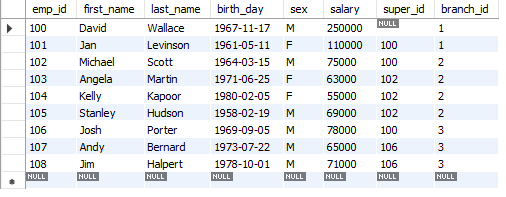
\includegraphics[width=0.4\textwidth]{./Figs/2020-12-24-20-38-38.png}
        % 	\caption{}
        \end{figure}
    
    \item Find all the clients:
        \begin{minted}[autogobble]{sql}
            SELECT * FROM client;
        \end{minted}
        \begin{figure}[H]
            \centering
            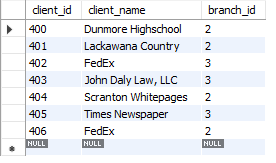
\includegraphics[width=0.4\textwidth]{./Figs/2020-12-24-20-39-09.png}
        % 	\caption{}
        \end{figure}
    
    \item Find all employees ordered by salary:
        \begin{minted}[autogobble]{sql}
            SELECT * FROM employee ORDER BY salary; 
        \end{minted}
        \begin{figure}[H]
            \centering
            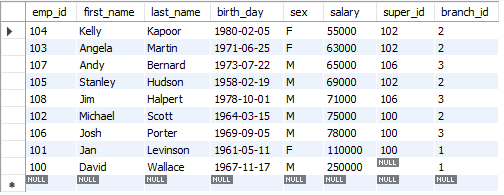
\includegraphics[width=0.4\textwidth]{./Figs/2020-12-24-20-39-36.png}
        % 	\caption{}
        \end{figure}
    
    \item Find all employees ordered by salary from largest to smallest and then smallest to largest:
        \begin{minted}[autogobble]{sql}
            SELECT * FROM employee ORDER BY salary DESC;
        \end{minted}
        \begin{figure}[H]
            \centering
            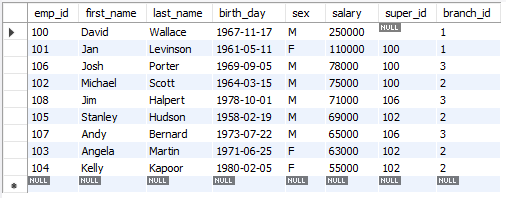
\includegraphics[width=0.4\textwidth]{./Figs/2020-12-24-20-44-00.png}
        % 	\caption{}
        \end{figure}
        \begin{minted}[autogobble]{sql}
            SELECT * FROM employee ORDER BY salary ASC;
        \end{minted}
        \begin{figure}[H]
            \centering
            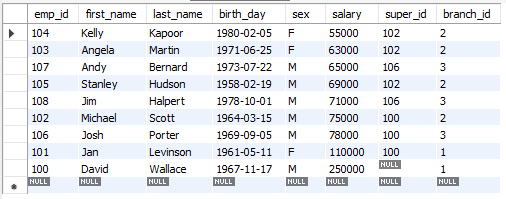
\includegraphics[width=0.4\textwidth]{./Figs/2020-12-24-20-44-41.png}
        % 	\caption{}
        \end{figure}
    
    \item Order all employees ordered by sex and then name:
        \begin{minted}[autogobble]{sql}
            SELECT * FROM employee ORDER BY sex, first_name, last_name; 
        \end{minted}
        \begin{figure}[H]
            \centering
            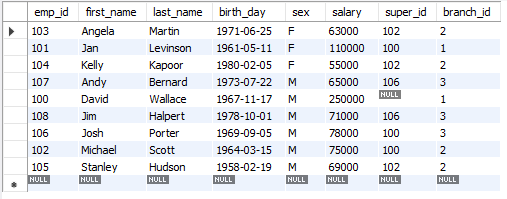
\includegraphics[width=0.4\textwidth]{./Figs/2020-12-24-20-43-11.png}
        % 	\caption{}
        \end{figure}
    
    \item Find the first 5 employees in the table:
        \begin{minted}[autogobble]{sql}
            SELECT * FROM employee LIMIT 5;
        \end{minted}
        \begin{figure}[H]
            \centering
            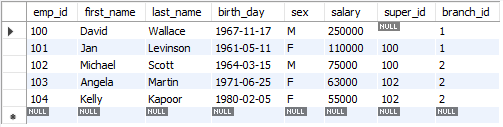
\includegraphics[width=0.4\textwidth]{./Figs/2020-12-24-20-45-25.png}
        % 	\caption{}
        \end{figure}
    
    \item Find the first and last names of all employees:
        \begin{minted}[autogobble]{sql}
            SELECT first_name, last_name FROM employee;
        \end{minted}
        \begin{figure}[H]
            \centering
            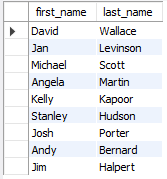
\includegraphics[width=0.4\textwidth]{./Figs/2020-12-24-20-45-46.png}
        % 	\caption{}
        \end{figure}
    
    \item  Find the forename and surnames of all employees:
        \begin{minted}[autogobble]{sql}
            SELECT first_name AS forename, last_name AS surname FROM employee;
        \end{minted}
        \begin{figure}[H]
            \centering
            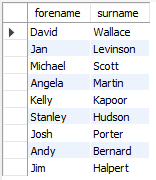
\includegraphics[width=0.4\textwidth]{./Figs/2020-12-24-20-46-18.png}
        % 	\caption{}
        \end{figure}
        \begin{itemize}
            \item \mintinline{sql}{AS} Allows you to select the columns differently to their names.
        \end{itemize}
    
    \item Find out all the different genders:
        \begin{minted}[autogobble]{sql}
            SELECT  DISTINCT sex FROM employee;
        \end{minted}
        \begin{figure}[H]
            \centering
            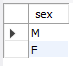
\includegraphics[width=0.4\textwidth]{./Figs/2020-12-24-20-46-37.png}
        % 	\caption{}
        \end{figure}
        \begin{itemize}
            \item \mintinline{sql}{DISTINCT} allows you to know all the values stored in a column. 
        \end{itemize}
    
    \item Find all male employees:
        \begin{minted}[autogobble]{sql}
            SELECT * FROM employee WHERE sex = 'M';
        \end{minted}
        \begin{figure}[H]
            \centering
            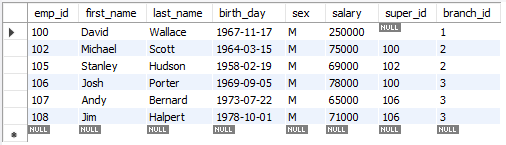
\includegraphics[width=0.4\textwidth]{./Figs/2020-12-24-20-47-19.png}
        % 	\caption{}
        \end{figure}
    
    \item Find all employees at branch 2:
        \begin{minted}[autogobble]{sql}
            SELECT * FROM employee WHERE branch_id = 2;
        \end{minted}
        \begin{figure}[H]
            \centering
            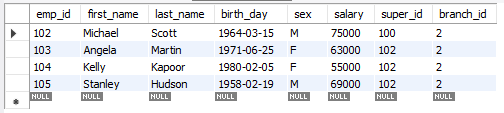
\includegraphics[width=0.4\textwidth]{./Figs/2020-12-24-20-48-13.png}
        % 	\caption{}
        \end{figure}
    
    \item Find all employee's id's and names who were born after 1969:
        \begin{minted}[autogobble]{sql}
            SELECT emp_id, first_name, last_name FROM employee WHERE birth_day >= 1970-01-01;
        \end{minted}
        \begin{figure}[H]
            \centering
            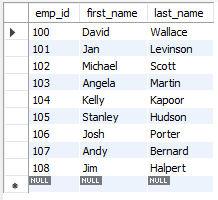
\includegraphics[width=0.4\textwidth]{./Figs/2020-12-24-20-48-48.png}
        % 	\caption{}
        \end{figure}
    
    \item Find all female employees at branch 2:
        \begin{minted}[autogobble]{sql}
            SELECT * FROM employee WHERE branch_id = 2 AND sex = 'F';
        \end{minted}
        \begin{figure}[H]
            \centering
            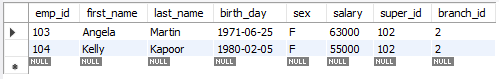
\includegraphics[width=0.4\textwidth]{./Figs/2020-12-24-20-49-50.png}
        % 	\caption{}
        \end{figure}
    
    \item Find all employees who are female  \& born after 1969 or who make over 80000:
        \begin{minted}[autogobble]{sql}
            SELECT * FROM employee WHERE (birth_day >= '1970-01-01' AND sex = 'F') OR salary > 80000;
        \end{minted}
        \begin{figure}[H]
            \centering
            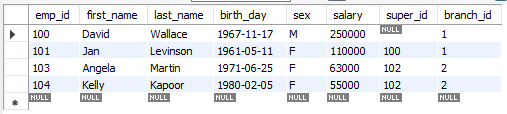
\includegraphics[width=0.4\textwidth]{./Figs/2020-12-24-20-50-39.png}
        % 	\caption{}
        \end{figure}
    
    \item Find all employees born between 1970 and 1975:
        \begin{minted}[autogobble]{sql}
            SELECT * FROM employee WHERE birth_day BETWEEN '1970-01-01' AND '1975-01-01';
        \end{minted}
        \begin{figure}[H]
            \centering
            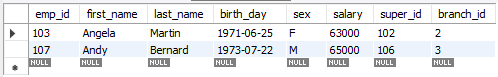
\includegraphics[width=0.4\textwidth]{./Figs/2020-12-24-20-51-24.png}
        % 	\caption{}
        \end{figure}
    
    \item Find all employees named Jim, Michael, Johnny or David:
        \begin{minted}[autogobble]{sql}
            SELECT * FROM employee WHERE first_name IN ('Jim', 'Michael', 'Johnny', 'David');
        \end{minted}
        \begin{figure}[H]
            \centering
            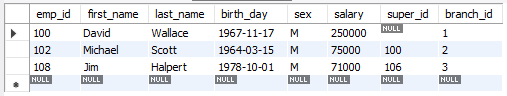
\includegraphics[width=0.4\textwidth]{./Figs/2020-12-24-20-52-10.png}
        % 	\caption{}
        \end{figure}
\end{itemize}



\chapter{Advanced Python Objects and Data Structures}
\section{Prompts to functions}
\begin{itemize}
    \item Find the number of employees are inside the employee table:
        \begin{minted}[autogobble]{sql}
            SELECT COUNT(emp_id) FROM employee;
        \end{minted}
    
    \item Find how many employees have supervisors:
        \begin{minted}[autogobble]{sql}
            SELECT COUNT(super_id) FROM employee;
        \end{minted}
    
    \item Find the number of female employees born after 1970:
        \begin{minted}[autogobble]{sql}
            SELECT COUNT(emp_id) FROM employee WHERE sex = 'F' AND birth_date > '1971-01-01';
        \end{minted}
    
    \item Find the average of all employee's salaries:
        \begin{minted}[autogobble]{sql}
            SELECT AVG(salary) FROM employee;
        \end{minted}
    
    \item Find the average of all employee's salaries who are male:
        \begin{minted}[autogobble]{sql}
            SELECT AVG(salary) FROM employee WHERE sex = 'M';
        \end{minted}
    
    \item Find the sum of all employee's salaries:
        \begin{minted}[autogobble]{sql}
            SELECT SUM(salary) FROM employee;
        \end{minted}
    
    \item Find out how many males and how many females there are:
        \begin{minted}[autogobble]{sql}
            SELECT COUNT(sex), sex FROM employee GROUP BY sex;
        \end{minted}
        \begin{itemize}
            \item This is called aggregation.
            \item The \mintinline{sql}{GROUP BY} allows us to display the count(sex) and sex in columns so that we can see what number belongs to what.
        \end{itemize}
    
    \item Find the total sales of each salesman:
        \begin{minted}[autogobble]{sql}
            SELECT SUM(total_sales), emp_id FROM works_with GROUP BY emp_id;
        \end{minted}
    
    \item Find the total purchases made from clients:
        \begin{minted}[autogobble]{sql}
            SELECT SUM(total_sales), emp_id FROM works_with GROUP BY client_id;
        \end{minted}
\end{itemize}


%%%%%%%%%%%%%%%%%%%%%%%%%%%%%%%%%%%%%%%%%%%%%%%%%%%%%%%%%%%%%%%%%%%%%%%%%%%%%%%%%%%%%%%%%%%%%%%%%%%%%%%%%%%%%%%%%%%%%%%%%%%%%%%%%%%%%%%%%%%%%%
\end{document}

